\documentclass{article}
\usepackage{amsmath}
\usepackage{enumitem}
\usepackage{amssymb}
\usepackage{tikz}
\usepackage{bbm}
\usepackage{geometry}
\usepackage{mathtools}
\usepackage{amsthm}
\usepackage{graphicx}
\DeclareMathOperator*{\argmin}{arg\!\min}
\DeclareMathOperator*{\argmax}{arg\!\max}

\geometry{letterpaper, portrait, margin=1in}
\newcommand{\ul}[0]{\underline}
\newcommand{\hs}[1]{\hspace*{#1 cm}}
\newcommand{\ind}[0]{\indent}
\newcommand{\tx}[1]{\text{#1}}

\newtheorem{theorem}{Theorem}[section]
\newtheorem{corollary}{Corollary}[theorem]
\newtheorem{lemma}[theorem]{Lemma}
\newtheorem{remark}{Remark}



\title{Homework \# }
\author{Derek Modzelewski}

\begin{document}

\maketitle

\section{Overview}

\subsection{Abstract} %@[nch]
\hs{.5}
For all tissues in our dataset, gene expression has some spread around the centroid for that tissue. We will attempt to answer if this spread can be related in a linear manner between many tissues. Essentially, whether or not the spread around one tissue can be modeled by a linear transform of the spread around another tissue.

This is equivalent to giving each patient a vector representation, and each tissue a linear transform from those vectors to gene expression.

\subsection{Possible implications}
\hs{.5}
Since we are giving each patient a vector representation in a shared, low dimensional space, this model will allow direct and efficient comparisons between patients. For example, a linear classifier could be trained on patient representations returned from our model. Without our model, it is extremely hard to compare patients at all since it is very likely that no two patients have samples for exactly the same set of tissues.  \\

Also, our model can be used to predict gene expressions. This could be used to fill in gaps of any dataset, ensuring that every patient has data in every tissue, albeit some predicted instead of measured, which may make other analyses much easier. It might also allow researchers to gain the same amount of information from fewer tissue samples, reducing costs. \\

\subsection{Related Work}
None to our knowledge.

\subsection{Data} %@[unf]
\hs{.5}
Our primary data is collection of gene expressions for roughly 300 patients across roughly 40 different tissues. %@[check]
It was acquired from "https://gtexportal.org/home/datasets", labeled 'GTEx\_Analysis\_v6p\_eQTL\_expression\_matrices.tar', and is about 2 gigabytes after uncompressing). Many patients have gene expression data for many distinct tissues, a fact which will be used heavily in our training. \\

We separated some of our data off for testing - ALL data from liver tissue samples, and 10\% of the patients from each of the other tissue types.


\section{Model} %@[nch]

\subsection{Notation} %@[unf]

For the rest of this paper:
\begin{align*}
Y_{iu} &:= \tx{Gene Expression for patient $u$ in tissue $i$, clarified below} \\
S_u &:= \tx{Euclidean vector representation of patient $u$} \\
h &:= \tx{Dimensionality of patient representations} \\
d &:= \tx{Dimensionality of expression representations} \\
F_i &:= \tx{Linear transform ($\mathbb{R}^{d \times h}$) associated with tissue $i$}
\end{align*}

In general, the variables $i,j$ will be reserved for indexing tissues, and $u,v$ will be reserved for indexing patients \\

As will be discussed later, it is useful to look at the difference of gene expression and tissue average:
\[ Y_{iu} = \tx{Gene Expression}_u - E[\tx{tissue}_i] \]
and $Y_i$ is a matrix including all patients $u$ for which we have data for tissue $i$, and every row sums to $0$ \\

\subsection{Generative Model}

All of our analysis is based on a model that:
\[ \tx{Gene Expression for patient $u$ in tissue $i$} \sim c(i) + F_i S_u + \mathcal{N}(0,\sigma^2) \]
where $c(i)$ is the mean for tissue $i$ across all patients, not just the ones for which we have data \\

Note that $d$ does not need to be the same for all tissues, since we apply a different PCA analysis for each tissue. Some of the equations later in this paper require that $h < d$ for all tissues, though. Later, we also use Bayesian Information Criterion to determine the optimal setting of $h$, which is $5$ \\ 


\section{Training} %@[unf]

Firstly, $\forall i$ we set $c(i)$ as the sample mean of the tissue's expressions. While $c(i)$ should be the actual mean instead of the sample mean, we expect this difference to be largely minimal and we were unable to find a clean solution for handling this difference. As shown by the graph 'Cerebellum\_x\_Lung.png", it is actually quite incorrect to assume $c(i)$ is the sample mean, and that is a possible future improvement. \\
This gives us:
\[ Y_{iu} = \tx{Gene Expression} - E[\tx{tissue } i] \sim F_i S_u + \mathcal{N}(0,\sigma^2) \]
Thus, $c(i)$ is not a parameter to be learned in training. \\
Using notation described in previous section:
\[ Y_i \sim F_i S + \mathcal{N}(0,\sigma^2) \]

Given $S$, solving for MLE is simple a least squares evaluation (as we saw in Linear Regression):
\begin{align*}
F_i &\leftarrow Y_i S^T\big(SS^T)^{-1} \hs{1}\forall i
\end{align*}

And when $F_i$ is held constant, least squares may also find optimal $S$ for tissue $i$, but we must simultaneously minimize the squared error for ALL tissues with $S$ \\

Our solution, which is not perfect, is to find the least squares solution for $S$ with each tissue, then average all of the values for each patient across all relevant tissues (for which the patient has data). \\
{\it i.e.} for each patient, where $I_u$ is the set of tissues for which patient $u$ has data:
\[ S_u \leftarrow \frac{1}{|I_u|}\sum_{i \in I_u} (F_i^TF_i)^{-1}F_i^T Y_{iu} \hs{1}\forall u\]

In training we will use these equations to implement an {\bf EM algorithm} to maximize the likelihood of the data given our initial model. We will alternate solving for $F$ and $S$, giving us an algorithm sketch:
\begin{enumerate}
\item Initialize $F$, $S$ randomly according to normal distribution
\item Repeat until convergence:
	\begin{enumerate}
	\item set $F_i \leftarrow Y_i S^T\big(SS^T)^{-1} \hs{1}\forall i$
	\item set $S_u \leftarrow \frac{1}{|I_u|}\sum_{i \in I_u} (F_i^TF_i)^{-1}F_i^T Y_{iu} \hs{1}\forall u$
	\end{enumerate}
\end{enumerate}


\section{Results}

\subsection{Plotting patients in one tissue vs another tissue}

Due to the linear nature of our model, if two patients in the same tissue have opposite displacement from the center, they must have opposite representations (sum to 0). This property must hold for all tissues which also contain those two patients. \\

To hopefully demonstrate this effect, we took the plot of the Cerebellum expressions (an arbitrary tissue) across the first two principle components. We labeled patients in the first quadrant as red, the second quadrant as purple, the third quadrant as green, and the fourth quadrant as blue. See 'Cerebellum\_x\_Cerebellum.png'. Thus, in the Cerebellum tissue, red patients have opposite displacement as green patients, and purple patients have opposite displacement as blue patients (with a lot of error as we are losing a lot of information when projecting two only two dimensions). We would then expect, as much as we can with only two dimensions, that in other tissues, red patients are opposite green patients and blue are oppsite purple. As shown in 'Cerebellum\_x\_Frontal\_Cortex.png' and 'Cerebellum\_x\_Cortex.png', this pattern is mostly true. This shows that there is at least some linear relation between gene expressions for different tissues for each patient. This relation would be enough to say that our linear model has some validity. \\

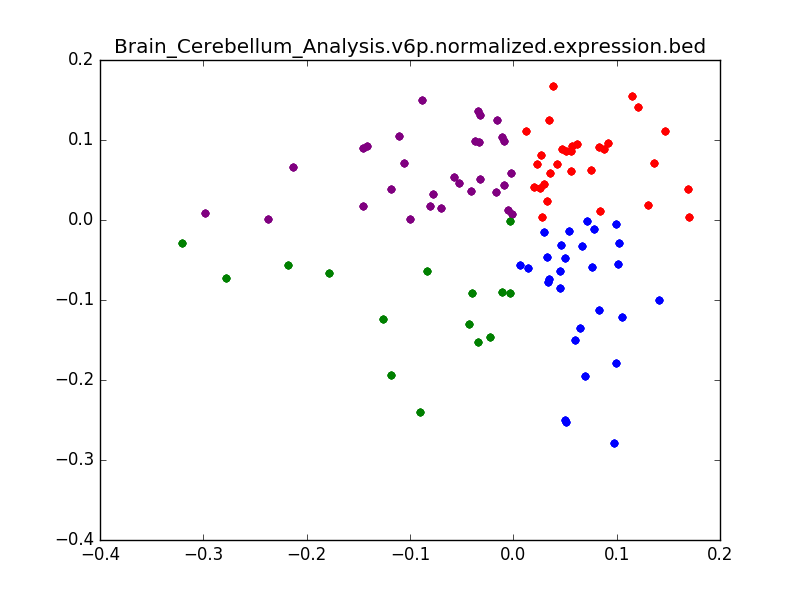
\includegraphics[scale = 0.6]{Cerebellum_x_Cerebellum}
Above - demonstrates how we are coloring patients

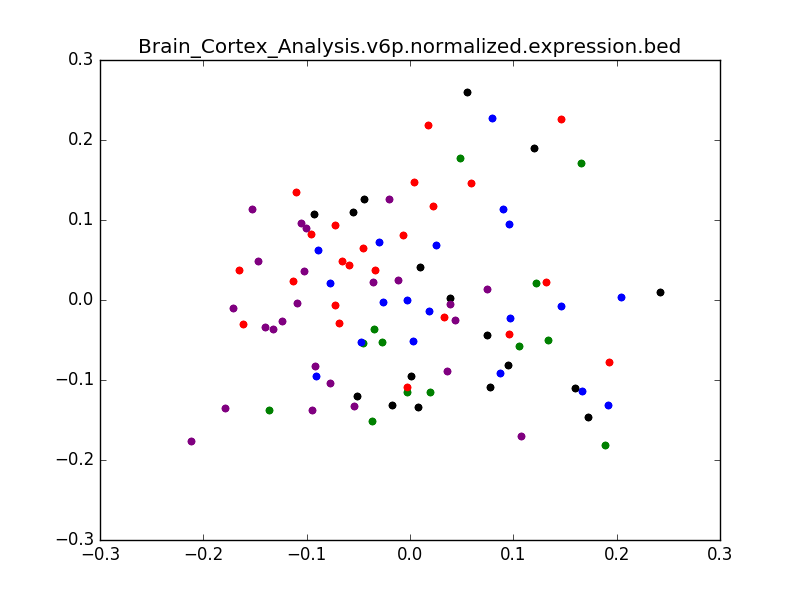
\includegraphics[scale = 0.6]{Cerebellum_x_Cortex}
Upon inspection, as in the original Cerebellum plot, red patients are generally on the opposite side of the origin from green patients, and blue patients are opposite purple patients.

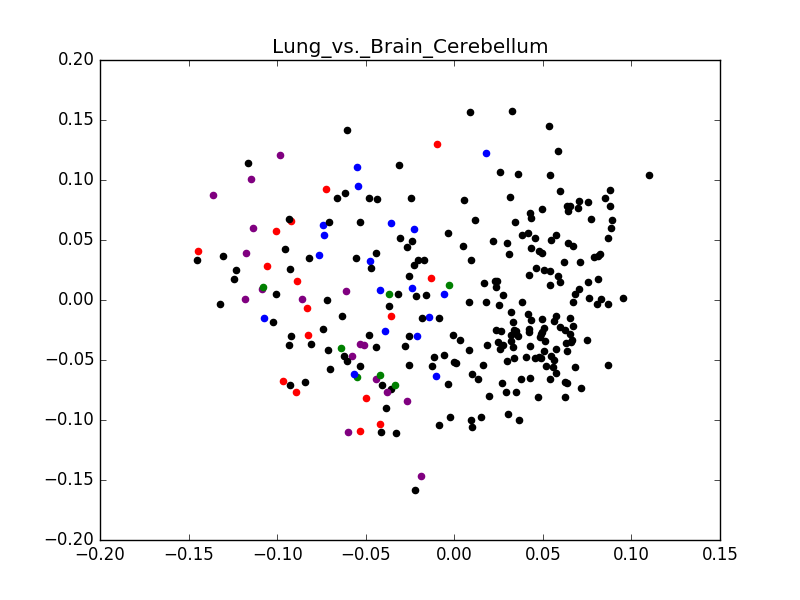
\includegraphics[scale = 0.8]{Cerebellum_x_Lung}
if the origin were at the center of the colored dots, the analysis would be correct that red patients are opposite green. Instead, all of the colored dots are on one side of the sample origin, so it is impossible for red and green patients to have opposite representations. This dynamic cannot be captured by our model, but still shows some linear structure. Thus, {\it we expect there to be more linear structure than our final results (simply based on our algorithm) will suggest}.

{\bf Takeaway}: Visually, it seems like our model captures some of the structure of the data. We will see if our algorithm can also capture that structure. \\

\subsection{BIC values}
Recall:
\[ \tx{BIC} = \ln(n)k - 2 \ln p(Y | \theta) \]
Our data points are really the patients, for which we have information on several tissues, but the real datapoint is the patient:
\[ n = |\tx{patients}| = 446 \]
Once we determine $S$, the representations of the patients, $F$ is determined. $\therefore$ $S$ is the only true free parameter with dimension $h|\tx{patients}|$. Furthermore, note that for any distance-preserving linear transform (rotation), $R$, $FS = FR^{-1}RS = F' RS$ $\therefore$ the final predictions are equivalent. Thus, the actual free parameters is the free parameters in $S$ minus the free parameters in $R$, giving us
\[ k = |\tx{patients}|h - h = (|\tx{patients}|-1)h  = 445h\]
And $p(Y | \theta)$ is determined according to the model, where the error model is a random normal with optimal variance for maximizing likelihood. \\
See 'BIC\_Scores.png' for results \\
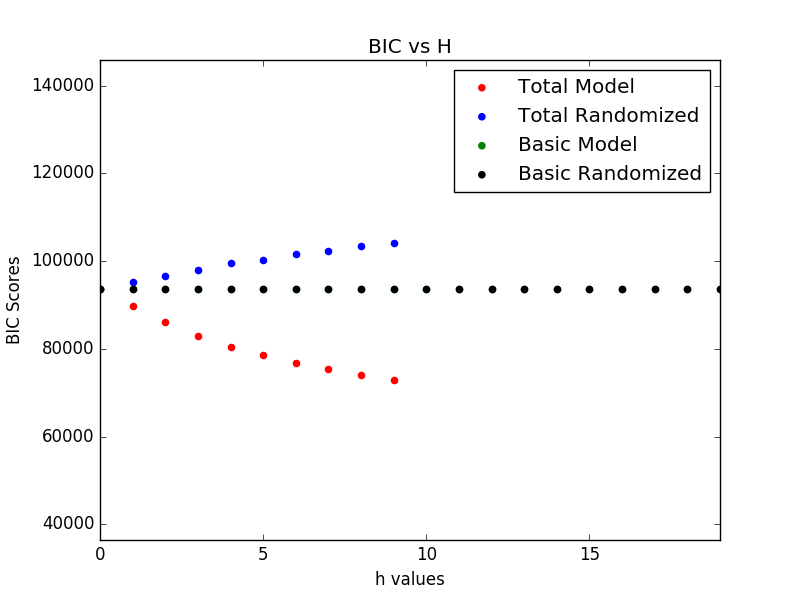
\includegraphics[scale = 0.6]{BIC_Scores.png}

From the plot, BIC is minimized at $h = 5$

\subsection{Variance explained}
See 'SSD\_plot.png' for plot of sum of squared error vs. $h$ hyperparameter. At the optimal $h$ setting, determined from minimizing BIC, the SSD is 240.7, whereas SSD is 340 when using the trivial model of simply predicting the centroids of each tissue for every patient (same behavior as when $h = 0$). Thus, our model explains $\frac{340 - 241.33}{340} = 29.0\%$ of the variance in the data. \\
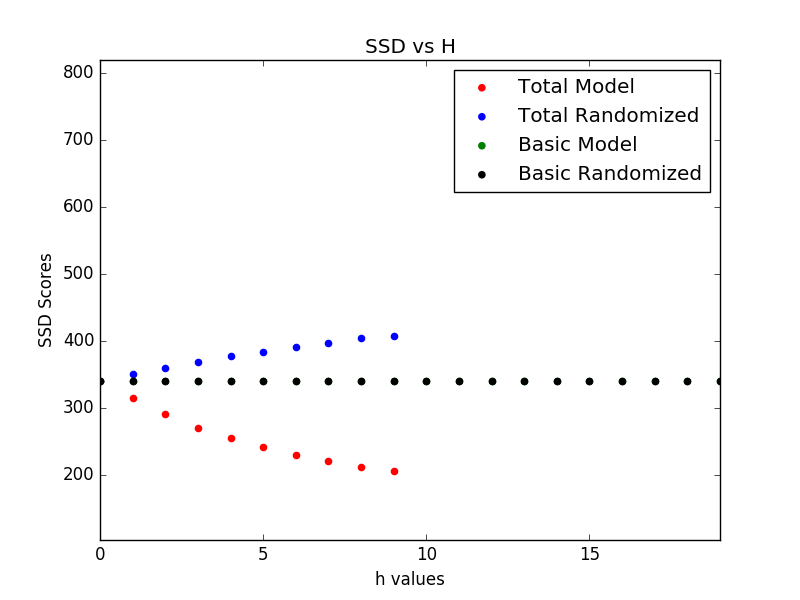
\includegraphics[scale = 0.6]{SSD_Scores.png}

This plot also solidifies our claim that our model is appropriate for the data. When our model is run on random data of the same form, the algorithm is only able to explain a small portion of the variance (seen in the blue series). When our model is run on the real data (the red series), though, it captures much more of the variance, showing that the data has far more linear structure than is expected. \\


\section{Conclusions} %@[unf]

\subsection{Goodness of model}
From the initial plots where we colored patients by quadrant in one tissue, it seemed like the data followed our model to a moderate degree. This is supported by the SSD plot. As shown, our algorithm learns the structure of the actual data set much better than it learns the structure of random data. (Roughly twice as much variance explained.)

Thus, our model is applicable and demonstrates some of the underlying structure of the data.

\subsection{Uses of model}
\hs{1}

{\bf Filling gaps in data}: For any patient, $u$, with data in other tissues, we can use our model to predict the expression of that patient in any other tissue. \\
Since we have data for other tissues, we have a trained $S_u$ representation, and we have a $F_i$ transform for every tissue. Thus, even when we do not have data for patient $u$ with tissue $i$, we can model it with $Y_{iu} \approx F_i S_u$ \\

{\bf Comparing patients}: We can use the representations of patients themselves to compare patients to patients. \\
Without our analysis, it is rather difficult to compare patients. At best, given two patients, one could search through all tissues and compare the gene expressions for each patient in each tissue. This is prohibitively slow. With our analysis, however, one can simply compare the cosine similarity of the representations of the two patients' representations. If this similarity is near one, we expect the patients to have nearly the same gene expression in all tissues. If the cosine similarity is near negative one, we expect opposite expressions. These similarities could likely be used as correlates for ancestry and possibly even diagnosis. \\



\subsection{Future improvements}
\hs{1}

{\bf Redo analysis with different PCA}: In our analysis, we always used PCA to reduce each tissue's gene expression to 10 dimensions. This number need not be 10, in fact it may even vary by tissue (some tissues may have 5 dimensions, others 15). It seems reasonable to reduce the tissues with less data to fewer dimensions, and 10 is a very arbitrary number. If we had more time, we might compare different systems for applying this PCA. \\

{\bf Quantify confidence in predictions}: As shown in our labeling of Brain Cortex by patients' expression in Cerebellum tissue, some tissues share a lot of structure. On the other hand, other tissue pairs such as Cerebellum and Lung, there is less shared structure. Thus, if a patient has a lot of brain tissue samples, we should be more confident about predicting other brain tissue expressions, and less confident about unrelated tissues. This confidence rating could be very useful in further analyses, but we do not yet have a model for it.

{\bf Allowing $h > d$}: Currently, our training equations require that $h \leq d$, but a simple change requires $h \geq d$. We could put a switch statement so that our code can choose which equation to use based on the comparison of $h$ and $d$, thereby working for all $h$ and $d$. \\

{\bf Admitting that $c(i)$ is not the sample mean}: This assumption made our analysis significantly easier as we did not have to train $c$. We could probably use a similar algorithm, alternatively solving for $F$, then $S$, then $c$ instead of $F$ and $S$ to get better results and a better estimation of the true mean of each tissue. \\












%

\end{document}